\chapter[ESPACIOS VECTORIALES CON PRODUCTO INTERNO]{ESPACIOS VECTORIALES \\ CON PRODUCTO \\ INTERNO}

En los capítulos anteriores hemos desarrollado una base sólida para comprender la estructura de los espacios vectoriales y sus aplicaciones. Comenzamos con el estudio de los espacios vectoriales reales, donde se establecieron los principios fundamentales que rigen la combinación lineal, la independencia y las bases. Posteriormente, el análisis de las matrices nos permitió disponer de una herramienta algebraica para representar y manipular transformaciones, así como para organizar información de manera sistemática. La teoría de los determinantes añadió un componente crucial al dotarnos de un criterio para la invertibilidad de matrices y el cálculo de volúmenes orientados, ampliando la visión geométrica del álgebra lineal. Finalmente, las transformaciones lineales integraron todos estos conceptos, mostrando cómo las estructuras abstractas se reflejan en aplicaciones concretas, revelando la estrecha relación entre álgebra y geometría.

En este capítulo avanzamos un paso más hacia la comprensión profunda de los espacios vectoriales introduciendo la noción de producto interno. Esta operación enriquece la estructura algebraica con una dimensión geométrica adicional, permitiendo medir longitudes, calcular ángulos y definir ortogonalidad entre vectores. Gracias a ello, conceptos como la proyección ortogonal, la descomposición en subespacios y la noción de ortonormalidad cobran sentido matemático y aplicación práctica. Así, los espacios vectoriales con producto interno constituyen el puente natural entre el álgebra lineal y la geometría euclidiana.

\newpage

Algunos ejemplos comunes de espacios vectoriales con producto interno incluyen espacios espacios de funciones, donde los vectores son funciones y el producto interno puede ser definido utilizando la integral de su producto puntual, y espacios de matrices, donde los vectores son matrices y el producto interno puede ser definido de diversas maneras, como el producto de Frobenius.

\section{Producto punto, norma y proyecciones}\label{sec:orto}

En este texto denotaremos la longitud de un vector $\mathbb{u}$ por el símbolo $\|\mathbb{u}\|$, que se lee como la \emph{norma} de $\mathbb{u}$, la \emph{longitud} de $\mathbb{u}$ o la \emph{magnitud} de $\mathbb{u}$ (el término “norma” siendo un sinónimo matemático común para longitud). Como se sugiere en la Figura 3.2.1a, se deduce del Teorema de Pitágoras que la norma de un vector $\mathbb{u}$ en $\RR[2]$ es
\begin{equation}
    \|\mathbb{u}\| = \sqrt{u_1^2 + u_2^2}. \label{normaexp2}
\end{equation}
De manera similar, para un vector $\mathbb{u}$ en $\RR[3]$, se deduce de la Figura 3.2.1b y dos aplicaciones del Teorema de Pitágoras que
$$\|\mathbb{u}\|^2 = (OR)^2 + (RP)^2 = (OQ)^2 + (QR)^2 + (RP)^2 = u_1^2 + u_2^2 + u_3^2$$
y de ahí que
\begin{equation}
    \|\mathbb{u}\| = \sqrt{u_1^2 + u_2^2 + u_3^2}. \label{normaexp3}
\end{equation}
Motivados por el patrón de las fórmulas \eqref{normaexp2} y \eqref{normaexp3}, hacemos la siguiente definición.

\begin{definicion}{}{}
    Si $\mathbb{u}$ es un vector en $\RR[n]$, entonces la \emph{norma} de $\mathbb{u}$ (también llamada la \emph{longitud} de $\mathbb{u}$ o la \emph{magnitud} de $\mathbb{u}$) se denota por $\|\mathbb{u}\|$ y se define por la fórmula
    $$\|\mathbb{u}\| = \sqrt{u_1^2 + u_2^2 + \cdots + u_n^2}.$$
\end{definicion}

Recordando la definición \ref{definicion:JUNSJSNSN} del producto punto, si $\mathbb{u}$ es un vector en $\RR[n]$, entonces la norma puede expresarse en términos del producto punto como
$$\|\mathbb{u}\| = \sqrt{\mathbb{u} \bullet \mathbb{u}}.$$
En el siguiente teorema, se presentan algunas propiedades de la norma de un vector.

\begin{theorem}{}{propiedades_norma}
    Si $\mathbb{u}$ es un vector en $\RR[n]$, y si $k$ es un escalar, entonces
    \begin{enumerate}[label=\alph*), topsep=6pt, itemsep=0pt]
        \item $\| \mathbb{u} \| \geq 0$.
        \item $\| \mathbb{u} \| = 0$ si y solo si $\mathbb{u} = \mathbb{0}$.
        \item $\| k \mathbb{u} \| = |k| \| \mathbb{u} \|$.
    \end{enumerate}

    \tcblower
    \demostracion Dado que las propiedades (a) y (b) son demostraciones directas, nos enfocaremos en demostrar la propiedad (c). Sea $\mathbb{u} \in \RR[n]$ y $k \in \RR$, entonces
    \begin{align*}
        \| k \mathbb{u} \|^2 & = (k \mathbb{u}) \bullet (k \mathbb{u}) \\
        & = k \big( \mathbb{u} \bullet (k \mathbb{u}) \big) \\
        & = k \cdot k (\mathbb{u} \bullet \mathbb{u}) \\
        & = k^2 \| \mathbb{u} \|^2
    \end{align*}
    De esta forma, $\| k \mathbb{u} \|^2 = k^2 \| \mathbb{u} \|^2$. Por el curso de Cálculo I, sabemos que $\sqrt{k^2} = |k|$. Así pues, se hereda que
    $$\big| \| k \mathbb{u} \| \big| = |k| \, \big| \| \mathbb{u} \| \big|.$$
    Finalmente, de la propiedad (a) de este teorema se sigue que
    $$\| k \mathbb{u} \| = |k| \| \mathbb{u} \|.$$
\end{theorem}

\newpage

Un vector de norma $1$ se llama \emph{vector unitario}. Estos vectores son útiles para especificar una dirección cuando la longitud no es relevante para el problema en cuestión. Se puede obtener un vector unitario en una dirección deseada eligiendo cualquier vector no nulo $\mathbb{u}$ en esa dirección y multiplicándolo por el recíproco de su longitud. Es decir, si $\mathbb{u}$ es cualquier vector no nulo en $\RR[n]$, entonces\infoBulle{A veces verás la fórmula \eqref{vectorunit} expresada como
$$\hat{\mathbb{u}} = \frac{\mathbb{u}}{\| \mathbb{u} \|}.$$
Esta es solo una forma más compacta de escribir dicha fórmula y no pretende dar a entender que el vector $\mathbb{u}$ esté siendo dividido por $\| \mathbb{u} \|$.}
\begin{equation}
    \hat{\mathbb{u}} = \frac{1}{\|\mathbb{u}\|} \mathbb{u} \label{vectorunit}
\end{equation}
define un vector unitario que está en la misma dirección que $\mathbb{u}$. Podemos confirmar que \eqref{vectorunit} es un vector unitario aplicando la parte (c) del teorema \ref{theorem:propiedades_norma} con $k = \dfrac{1}{\|\mathbb{u}\|}$ para obtener
$$\|\hat{\mathbb{u}}\| = \|k\mathbb{u}\| = |k| \|\mathbb{u}\| = k \|\mathbb{u}\| = \frac{1}{\|\mathbb{u}\|} \|\mathbb{u}\| = 1.$$
El proceso de multiplicar un vector $\mathbb{u} \neq \mathbb{0}$ por el recíproco de su norma para obtener un vector unitario $\hat{\mathbb{u}}$ se denomina \emph{normalización}.

\begin{examplebox}{}{}
    Normalice el siguiente vector:
    \begin{matrizn}
        \makecell{\includegraphics[page=1]{Externalizacion/C5/MatricesC5.pdf}}
    \end{matrizn}

    \tcblower
    \solucion La norma del vector $\mathbb{u}$ es
    $$\| \mathbb{u} \| = \sqrt{(-1)^2 + (2)^2 + (-4)^2 + (3)^2} = \sqrt{30}.$$
    Por lo tanto, al normalizar el vector $\mathbb{u}$, obtenemos que
    \begin{matrizn}
        \makecell{\includegraphics[page=2]{Externalizacion/C5/MatricesC5.pdf}}
    \end{matrizn}
    Se deja al lector confirmar que $\| \hat{\mathbb{u}} \| = 1$.
\end{examplebox}

El siguiente teorema proporciona propiedades adicionales del producto punto. Las demostraciones se dejan al lector y pueden obtenerse expresando los vectores en términos de componentes o utilizando las propiedades algebraicas establecidas en el teorema \ref{theorem:propiedadespunto1}.

\begin{theorem}{}{propiedadespunto2}
    Si $\mathbb{u}$, $\mathbb{v}$, $\mathbb{w}$ son vectores en $\RR[n]$, entonces
    \begin{enumerate}[label=\roman*), topsep=6pt, itemsep=0pt]
        \item $(\mathbb{u} + \mathbb{v}) \bullet \mathbb{w} = \mathbb{u} \bullet \mathbb{w} + \mathbb{v} \bullet \mathbb{w}$.
        \item $\mathbb{u} \bullet (\mathbb{v} - \mathbb{w}) = \mathbb{u} \bullet \mathbb{v} - \mathbb{u} \bullet \mathbb{w}$.
        \item $(\mathbb{u} - \mathbb{v}) \bullet \mathbb{w} = \mathbb{u} \bullet \mathbb{w} - \mathbb{v} \bullet \mathbb{w}$.
    \end{enumerate}
\end{theorem}

\begin{examplebox}{}{}
    Simplifique la siguiente expresión:
    $$(\mathbb{u} - 2\mathbb{v}) \bullet (3\mathbb{u} + 4\mathbb{v}).$$

    \tcblower
    \solucion Usando las propiedades de los teoremas \ref{theorem:propiedadespunto1} y \ref{theorem:propiedadespunto2},
    \begin{align*}
        (\mathbb{u} - 2\mathbb{v}) \bullet (3\mathbb{u} + 4\mathbb{v}) & = \mathbb{u} \bullet (3\mathbb{u} + 4\mathbb{v}) - 2\mathbb{v} \bullet (3\mathbb{u} + 4\mathbb{v}) \\
        & = 3(\mathbb{u} \bullet \mathbb{u}) + 4(\mathbb{u} \bullet \mathbb{v}) - 6(\mathbb{v} \bullet \mathbb{u}) - 8(\mathbb{v} \bullet \mathbb{v}) \\
        & = 3\| \mathbb{u} \|^2 - 2(\mathbb{u} \bullet \mathbb{v}) - 8\| \mathbb{v} \|^2
    \end{align*}
\end{examplebox}

\newpage

\begin{adjustwidth}{-7.6cm}{-2cm}
    \begin{tcolorbox}[
        theorem style=change break,
        enhanced,
        breakable,
        boxrule=0pt,
        frame hidden,
        left = 1.8cm,
        right = 1.8cm,
        top=4mm,
        bottom=2mm,
        colback=black!7!white,
        coltitle=black,
        attach title to upper={\ },
        sharp corners,
        borderline north={1.5pt}{0pt}{black},
        title = {Aplicación del producto punto a números ISBN},
        fonttitle=\selectfont\Lato\bfseries\LARGE,
        fontupper=\normalsize
    ]
        \begin{multicols}{2}
            Aunque el sistema ha cambiado recientemente, la mayoría de los libros antiguos han sido asignados un número único de 10 dígitos llamado Número Internacional Estándar de Libro o por sus siglas en inglés, ISBN (\emph{International Standard Book Number}). Los primeros nueve dígitos de este número se dividen en tres grupos: el primer grupo representa el país o grupo de países en los que se originó el libro, el segundo identifica al editor, y el tercero está asignado al título del libro mismo. El décimo y último dígito, llamado dígito de control, se computa a partir de los primeros nueve dígitos y se usa para asegurar que una transmisión electrónica del ISBN, digamos a través de Internet, ocurra sin error. Para explicar cómo se hace esto, consideremos los primeros nueve dígitos del ISBN como un vector $\mathbb{b}$ en $\RR[9]$, y dejemos que $\mathbb{a}$ sea el vector
            \begin{matrizn}
                \makecell{\includegraphics[page=3]{Externalizacion/C5/MatricesC5.pdf}}
            \end{matrizn}
            Entonces, el dígito de control $c$ se computa usando el siguiente procedimiento:\vspace{0.3cm}
            \begin{enumerate}[label=\roman*)]
                \item Formar el producto punto $\mathbb{a} \bullet \mathbb{b}$.
                \item Dividir $\mathbb{a} \bullet \mathbb{b}$ entre 11, produciendo un resto $c$ que es un entero entre 0 y 10, inclusive. El dígito de control se toma como $c$, con la salvedad de que $c = 10$ se escribe como X para evitar dígitos dobles.\vspace{0.3cm}
            \end{enumerate}
            Por ejemplo, el ISBN del libro \emph{Álgebra Lineal}, quinta edición, de Stanley I. Grossman es
            $$970-10-0890-1$$
            que tiene un dígito de control de $1$. Esto es consistente con los primeros nueve dígitos del ISBN, ya que
            \begin{matrizn}
                \makecell{\includegraphics[page=4]{Externalizacion/C5/MatricesC5.pdf}}
            \end{matrizn}
            Dividiendo $155$ entre $11$ produce un cociente de $14$ y un resto de $1$, por lo que el dígito de control es $c = 1$. Si se realiza un pedido electrónico de un libro con un cierto ISBN, el almacén puede usar el procedimiento anterior para verificar que el dígito de control es consistente con los primeros nueve dígitos, reduciendo así la posibilidad de un costoso error de envío.
        \end{multicols}
    \end{tcolorbox}
\end{adjustwidth}

Nuestro próximo objetivo es redefinir el producto punto sobre vectores en $\RR[2]$ y $\RR[3]$ y luego extender esa definición a $\RR[n]$. Para hacerlo, primero necesitamos definir exactamente qué queremos decir con el “ángulo” entre dos vectores en $\RR[2]$ o $\RR[3]$. Para este propósito, dejemos que $\mathbb{u}$ y $\mathbb{v}$ sean vectores no nulos en $\RR[2]$ o $\RR[3]$ que han sido posicionados de modo que sus puntos iniciales coincidan. Definimos el ángulo entre $\mathbb{u}$ y $\mathbb{v}$ como el ángulo $\theta$ determinado por $\mathbb{u}$ y $\mathbb{v}$ que satisface $0 \leq \theta \leq \pi$.
\begin{figure*}[h]
    \centering
    \subfloat[]{
    \begin{tikzpicture}
        \coordinate (O) at (0,0);
        \coordinate (V) at (2.25,0);
        \coordinate (U) at (45:2.25);
        %
        \draw[thick,-Latex] (O) -- (V) node[below left] {$\mathbb{v}$};
        \draw[thick,-Latex] (O) -- (U) node[below left,xshift=-8pt] {$\mathbb{u}$};
        %
        \pic[draw, -latex, "$\theta$", angle eccentricity=1.5] {angle = V--O--U};
    \end{tikzpicture}
    } \hfill
    \subfloat[]{
    \begin{tikzpicture}
        \coordinate (O) at (0,0);
        \coordinate (V) at (2.25,0);
        \coordinate (U) at (130:2.25);
        %
        \draw[thick,-Latex] (O) -- (V) node[below left] {$\mathbb{v}$};
        \draw[thick,-Latex] (O) -- (U) node[below left] {$\mathbb{u}$};
        %
        \pic[draw, -latex, "$\theta$", angle eccentricity=1.5] {angle = V--O--U};
    \end{tikzpicture}
    } \hfill
    \subfloat[]{
    \begin{tikzpicture}
        \coordinate (O) at (0,0);
        \coordinate (V) at (2.25,0);
        \coordinate (U) at (180:2.25);
        %
        \draw[thick,-Latex] (O) -- (V) node[below left] {$\mathbb{v}$};
        \draw[thick,-Latex] (O) -- (U) node[below right] {$\mathbb{u}$};
        %
        \pic[draw, -latex, "$\theta$", angle eccentricity=1.5] {angle = V--O--U};
    \end{tikzpicture}
    } \hfill
    \subfloat[]{
    \begin{tikzpicture}
        \coordinate (O) at (0,0);
        \coordinate (V) at (2.25,0);
        \coordinate (U) at (220:2.25);
        %
        \draw[thick,-Latex] (O) -- (V) node[below left] {$\mathbb{v}$};
        \draw[thick,-Latex] (O) -- (U) node[below right] {$\mathbb{u}$};
        %
        \pic[draw, -latex, "$\theta$", angle eccentricity=1.5] {angle = U--O--V};
    \end{tikzpicture}
    }
    \caption{El ángulo $\theta$ entre $\mathbb{u}$ y $\mathbb{v}$ satisface $0 \leq \theta \leq \pi$}
\end{figure*}

De acuerdo con la ley de cosenos, tenemos que
\begin{equation}
    \| \mathbb{u} - \mathbb{v} \|^2 = \| \mathbb{u} \|^2 + \| \mathbb{v} \|^2 - 2 \| \mathbb{u} \| \| \mathbb{v} \| \cos \theta. \label{primeroya}
\end{equation}
Ahora bien,
\begin{align*}
    \| \mathbb{u} - \mathbb{v} \|^2 & = (\mathbb{u} - \mathbb{v}) \bullet (\mathbb{u} - \mathbb{v}) \\
    & = \mathbb{u} \bullet (\mathbb{u} - \mathbb{v}) + (-\mathbb{v}) \bullet (\mathbb{u} - \mathbb{v}) \\
    & = \| \mathbb{u} \|^2 - 2(\mathbb{u} \bullet \mathbb{v}) + \| \mathbb{v} \|^2
\end{align*}

\newpage\noindent
Por lo tanto,
\begin{equation}
    \| \mathbb{u} - \mathbb{v} \|^2 = \| \mathbb{u} \|^2 - 2(\mathbb{u} \bullet \mathbb{v}) + \| \mathbb{v} \|^2. \label{segundoya}
\end{equation}
Igualando ambas expresiones \eqref{primeroya} y \eqref{segundoya},
$$\| \mathbb{u} \|^2 + \| \mathbb{v} \|^2 - 2 \| \mathbb{u} \| \| \mathbb{v} \| \cos \theta = \| \mathbb{u} \|^2 - 2(\mathbb{u} \bullet \mathbb{v}) + \| \mathbb{v} \|^2.$$
Entonces,
\begin{equation}
    \mathbb{u} \bullet \mathbb{v} = \| \mathbb{u} \| \| \mathbb{v} \| \cos \theta. \label{productopuntocos23}
\end{equation}
El signo del producto punto revela información sobre el ángulo $\theta$ que podemos obtener reescribiendo la fórmula \eqref{productopuntocos23} como
\begin{equation}
    \cos \theta = \frac{\mathbb{u} \bullet \mathbb{v}}{\|\mathbb{u}\| \|\mathbb{v}\|}. \label{angulovect23}
\end{equation}
Dado que $0 \leq \theta \leq \pi$, se deduce de la fórmula \eqref{angulovect23} y las propiedades de la función coseno estudiadas en trigonometría que
$$\theta \text{ es agudo si } \mathbb{u} \bullet \mathbb{v} > 0, \quad \theta \text{ es obtuso si } \mathbb{u} \bullet \mathbb{v} < 0, \quad \theta = \frac{\pi}{2} \text{ si } \mathbb{u} \bullet \mathbb{v} = 0.$$

\begin{examplebox}{}{}
    Encuentre el producto punto de los vectores que se muestran en la figura \ref{productopconcos}.

    \tcblower
    \solucion La norma de los vectores son
    $$\| \mathbb{u} \| = \sqrt{0^2 + 2^2} = 2, \qquad \| \mathbb{v} \| = \sqrt{2^2 + 2^2} = \sqrt{8} = 2\sqrt{2}$$
    y el coseno del ángulo $\theta$ entre ellos es
    $$\cos(45^{\circ}) = \frac{1}{\sqrt{2}}.$$
    Por lo tanto, se sigue de la fórmula \eqref{productopuntocos23} que
    $$\mathbb{u} \bullet \mathbb{v} = \| \mathbb{u} \| \| \mathbb{v} \| \cos \theta = (2) \left( 2\sqrt{2} \right) \left( \frac{1}{\sqrt{2}} \right) = 4.$$
\end{examplebox}
\sideFigure[\label{productopconcos}]{\vspace{-5cm}
\begin{tikzpicture}
    \coordinate (O) at (0,0);
    \coordinate (V) at (2,2);
    \coordinate (U) at (2,0);
    %
    \draw[thick,-Stealth] (-1,0) -- (4,0) node[above left] {$x$};
    \draw[thick,-Stealth] (0,-1) -- (0,4) node[below left] {$y$};
    %
    \draw[thick,-Latex] (O) -- (V) node[right] {$\mathbb{v} = \begin{pmatrix}
        2 \\
        2
    \end{pmatrix}$};
    \draw[thick,-Latex] (O) -- (U) node[below] {$\mathbb{u} = \begin{pmatrix}
        0 \\
        2
    \end{pmatrix}$};
    %
    \pic[draw, -, "$45^{\circ}$", angle eccentricity=1.6] {angle = U--O--V};
\end{tikzpicture}
}
Nuestro próximo objetivo es extender a $\RR[n]$ la noción de “ángulo” entre vectores no nulos $\mathbb{u}$ y $\mathbb{v}$. Haremos esto comenzando con la fórmula
\begin{equation}
    \theta = \arccos\left(\frac{\mathbb{u} \bullet \mathbb{v}}{\|\mathbb{u}\| \|\mathbb{v}\|}\right) \label{cosenoinvanguv}
\end{equation}
que previamente derivamos para vectores no nulos en $\RR[2]$ y $\RR[3]$. Dado que los productos puntos y las normas han sido definidos para vectores en $\RR[n]$, parecería que esta fórmula tiene todos los ingredientes para servir como definición del ángulo $\theta$ entre dos vectores $\mathbb{u}$ y $\mathbb{v}$ en $\RR[n]$. Sin embargo, hay un problema: el arcocoseno en la fórmula \eqref{cosenoinvanguv} no está definido a menos que su argumento satisfaga
\begin{equation}
    -1 \leq \frac{\mathbb{u} \bullet \mathbb{v}}{\|\mathbb{u}\| \|\mathbb{v}\|} \leq 1. \label{argumentodom}
\end{equation}
Afortunadamente, la expresión \eqref{argumentodom} es cierta para cualesquiera vectores no nulos en $\RR[n]$ como resultado de un resultado fundamental conocido como la \emph{desigualdad de Cauchy-Schwarz}.

\begin{theorem}{}{}
    \TituloBox{Desigualdad de Cauchy-Schwarz:} Si $\mathbb{u}$ y $\mathbb{v}$ son vectores en $\RR[n]$, entonces
    \begin{equation}
        |\mathbb{u} \bullet \mathbb{v}| \leq \|\mathbb{u}\| \|\mathbb{v}\| \label{CauchySchwarzRn}
    \end{equation}
    o en términos de componentes
    $$|u_1 v_1 + u_2 v_2 + \cdots + u_n v_n| \leq \left(u_1^2 + u_2^2 + \cdots + u_n^2\right)^{1/2} \left(v_1^2 + v_2^2 + \cdots + v_n^2\right)^{1/2}.$$
\end{theorem}

Omitiremos la demostración de este teorema porque más adelante en este capítulo probaremos una versión más general de la cual este será un caso especial. Nuestro objetivo por ahora será usar este teorema para probar que \eqref{argumentodom} se cumple para todos los vectores no nulos en $\RR[n]$. Una vez que esto se haya logrado, habremos establecido todos los resultados necesarios para usar la fórmula \eqref{cosenoinvanguv} como nuestra definición del ángulo entre vectores no nulos $\mathbb{u}$ y $\mathbb{v}$ en $\RR[n]$.

Para probar que la expresión \eqref{argumentodom} se cumple para todos los vectores no nulos en $\RR[n]$, dividimos ambos lados de la fórmula \eqref{CauchySchwarzRn} entre el producto $\|\mathbb{u}\| \|\mathbb{v}\|$ para obtener
$$\frac{|\mathbb{u} \bullet \mathbb{v}|}{\|\mathbb{u}\| \|\mathbb{v}\|} \leq 1 \quad \text{o equivalentemente} \quad \left|\frac{\mathbb{u} \bullet \mathbb{v}}{\|\mathbb{u}\| \|\mathbb{v}\|}\right| \leq 1$$
de lo cual \eqref{argumentodom} se deduce.

Las normas y el producto punto en $\RR[n]$ poseen relaciones fundamentales que conectan la geometría y el álgebra. El siguiente teorema resume identidades clave como la desigualdad del triángulo y la identidad del paralelogramo.

\begin{theorem}{}{}
    Si $\mathbb{u}$ y $\mathbb{v}$ son vectores en $\RR[n]$, entonces
    \begin{enumerate}[label=\roman*), topsep=6pt, itemsep=0pt]
        \item $\| \mathbb{u} + \mathbb{v} \| \leq \| \mathbb{u} \| + \| \mathbb{v} \|$. \hfill \eqtext{C}{(Desigualdad del triángulo)}
        \item $\| \mathbb{u} + \mathbb{v} \|^2 + \| \mathbb{u} - \mathbb{v} \|^2 = 2 \left( \| \mathbb{u} \|^2 + \| \mathbb{v} \|^2 \right)$. \hfill \eqtext{C}{(Identidad del paralelogramo)}
        \item $\| \mathbb{u} + \mathbb{v} \| \| \mathbb{u} - \mathbb{v} \| \leq \| \mathbb{u} \|^2 + \| \mathbb{v} \|^2$.
        \item $\mathbb{u} \bullet \mathbb{v} = \dfrac{1}{4} \left(\| \mathbb{u} + \mathbb{v} \|^2 - \| \mathbb{u} - \mathbb{v} \|^2\right)$. \hfill \eqtext{C}{(Identidad de polarización)}
    \end{enumerate}

    \tcblower
    \demostracion
    \begin{enumerate}[label=\roman*), topsep=6pt, itemsep=0pt]
        \item Sean $\mathbb{u}$ y $\mathbb{v}$ vectores en $\RR[n]$,
        \begin{align*}
            \| \mathbb{u} + \mathbb{v} \| & = (\mathbb{u} + \mathbb{v}) \bullet (\mathbb{u} + \mathbb{v}) \\
            & = (\mathbb{u} \bullet \mathbb{u}) + 2(\mathbb{u} \bullet \mathbb{v}) + (\mathbb{v} \bullet \mathbb{v}) \\
            & = \| \mathbb{u} \|^2 + 2(\mathbb{u} \bullet \mathbb{v}) + \| \mathbb{v} \|^2 \\
            & \leq \| \mathbb{u} \|^2 + 2|\mathbb{u} \bullet \mathbb{v}| + \| \mathbb{v} \|^2 \\
            & \leq \| \mathbb{u} \|^2 + 2 \| \mathbb{u} \| \| \mathbb{v} \| + \| \mathbb{v} \|^2 \\
            & = (\| \mathbb{u} \| + \| \mathbb{v} \|)^2
        \end{align*}
        \item Sean $\mathbb{u}$ y $\mathbb{v}$ vectores en $\RR[n]$,
        \begin{align*}
            \| \mathbb{u} + \mathbb{v} \|^2 + \| \mathbb{u} - \mathbb{v} \|^2 & = (\mathbb{u} + \mathbb{v}) \bullet (\mathbb{u} + \mathbb{v}) + (\mathbb{u} - \mathbb{v}) \bullet (\mathbb{u} - \mathbb{v}) \\
            & = 2(\mathbb{u} \bullet \mathbb{u}) + 2(\mathbb{v} \bullet \mathbb{v}) \\
            & = 2 \left( \| \mathbb{u} \|^2 + \| \mathbb{v} \|^2 \right)
        \end{align*}
        \item Sean $\mathbb{u}$ y $\mathbb{v}$ vectores en $\RR[n]$. Si definimos $a_1 = \| \mathbb{u} + \mathbb{v} \|^2$ y $a_2 = \| \mathbb{u} - \mathbb{v} \|^2$, observemos que podemos usar la \emph{desigualdad entre la media geométrica y la media aritmética} demostrada en el ejemplo \ref{examplebox:mediageometricaaritmetica}, pues $a_1$, $a_2 \geq 0$. De esta forma, obtenemos que
        $$\sqrt{\| \mathbb{u} + \mathbb{v} \|^2 \| \mathbb{u} - \mathbb{v} \|^2} \leq \frac{\| \mathbb{u} + \mathbb{v} \|^2 + \| \mathbb{u} + \mathbb{v} \|^2}{2},$$
        es decir,
        $$\| \mathbb{u} + \mathbb{v} \| \| \mathbb{u} - \mathbb{v} \| \leq \frac{\| \mathbb{u} + \mathbb{v} \|^2 + \| \mathbb{u} + \mathbb{v} \|^2}{2}.$$
        Pero por el inciso anterior, se obtiene finalmente que
        $$\| \mathbb{u} + \mathbb{v} \| \| \mathbb{u} - \mathbb{v} \| \leq \| \mathbb{u} \|^2 + \| \mathbb{v} \|^2.$$
        \item Se deja como ejercicio al lector.
    \end{enumerate}
\end{theorem}

\newpage

\begin{definicion}{}{vectores_ortonormales}
    Dados $\mathbb{u}_1$, $\mathbb{u}_2$, $\dots$, $\mathbb{u}_k \in \RR[n]$.
    \begin{enumerate}[label=\roman*), topsep=6pt, itemsep=0pt]
        \item Diremos que dos vectores $\mathbb{u}_i$ y $\mathbb{u}_j$ con $i \neq j$ son \emph{ortogonales} si $\mathbb{u}_i \bullet \mathbb{u}_j = 0$. En general, un conjunto $\left\{ \mathbb{u}_1, \mathbb{u}_2, \dots, \mathbb{u}_k \right\}$ se llama \emph{conjunto ortogonal} si todos sus vectores son ortogonales entre sí.
        \item Si además se cumple que cada $\mathbb{u}_i$ es un vector unitario, entonces los vectores se denominan \emph{ortonormales}, y el conjunto $\left\{ \mathbb{u}_1, \mathbb{u}_2, \dots, \mathbb{u}_k \right\}$ se llama \emph{conjunto ortonormal}.
    \end{enumerate}
\end{definicion}

\begin{examplebox}{}{}
    \begin{enumerate}[label=\roman*), topsep=6pt, itemsep=0pt]
        \item Considere los siguientes vectores
        \begin{matrizn}
            \makecell{\includegraphics[page=5]{Externalizacion/C5/MatricesC5.pdf}}
        \end{matrizn}
        Muestre que $\mathbb{u}$ y $\mathbb{v}$ son vectores ortogonales en $\RR[4]$.
        \item Sea $S = \{\mathbb{e}_1, \mathbb{e}_2, \mathbb{e_3}\}$ el conjunto de vectores estándar en $\RR[3]$. Muestre que el conjunto $S$ es un conjunto ortogonal.
    \end{enumerate}

    \tcblower
    \solucion
    \begin{enumerate}[label=\roman*), topsep=6pt, itemsep=0pt]
        \item Los vectores son ortogonales, ya que
        $$\mathbb{u} \bullet \mathbb{v} = (-2)(1) + (3)(2) + (1)(0) + (4)(-1) = 0.$$
        \item Es suficiente mostrar que
        $$\mathbb{e}_1 \bullet \mathbb{e}_2 = \mathbb{e}_1 \bullet \mathbb{e}_3 = \mathbb{e}_2 \bullet \mathbb{e}_3 = 0,$$
        porque se sigue del segundo inciso del teorema \ref{theorem:propiedadespunto1} que
        $$\mathbb{e}_2 \bullet \mathbb{e}_1 = \mathbb{e}_3 \bullet \mathbb{e}_1 = \mathbb{e}_3 \bullet \mathbb{e}_2 = 0.$$
        Por lo tanto
        \begin{align*}
            \mathbb{e}_1 \bullet \mathbb{e}_2 & = (1)(0) + (0)(1) + (0)(0) = 0 \\
            \mathbb{e}_1 \bullet \mathbb{e}_3 & = (1)(0) + (0)(0) + (0)(1) = 0 \\
            \mathbb{e}_2 \bullet \mathbb{e}_3 & = (0)(0) + (1)(0) + (0)(1) = 0
        \end{align*}
        lo que prueba que $S$ es un conjunto ortogonal.
    \end{enumerate}
\end{examplebox}

En muchas aplicaciones es necesario “descomponer” un vector $\mathbb{u}$ en la suma de dos términos, un término siendo un múltiplo escalar de un vector no nulo específico $\mathbb{v}$ y el otro término siendo ortogonal a $\mathbb{v}$. Por ejemplo, si $\mathbb{u}$ y $\mathbb{v}$ son vectores en $\RR[2]$ que están posicionados de modo que sus puntos iniciales coinciden en un punto $Q$, entonces podemos crear tal descomposición como sigue (figura \ref{posibles3casosproyort}):
\begin{itemize}
    \item Primero, consideremos la recta que pasa por el origen en la dirección del vector $\mathbb{v}$. Trazamos una perpendicular desde el extremo de $\mathbb{u}$ hasta dicha recta.
    \item A continuación, definimos el vector $\mathbb{w}_1$ como aquel que parte del punto inicial $Q$ y llega hasta el pie de la perpendicular construida en el paso anterior.
    \item Finalmente, definimos el vector $\mathbb{w}_2 = \mathbb{u} - \mathbb{w}_1$.
\end{itemize}
Dado que
$$\mathbb{w}_1 + \mathbb{w}_2 = \mathbb{w}_1 + (\mathbb{u} - \mathbb{w}_1) = \mathbb{u}$$
hemos descompuesto $\mathbb{u}$ en la suma de dos vectores ortogonales, el primer término siendo un múltiplo escalar de $\mathbb{v}$ y el segundo siendo ortogonal a $\mathbb{v}$.\sideFigure[Tres posibles casos\label{posibles3casosproyort}]{
\makecell[l]{
    \begin{tikzpicture}
        \coordinate (Q) at (0,0);
        \coordinate (W1) at (1.6,0);
        \coordinate (W2) at (0,1.6);
        \coordinate (U) at (1.6,1.6);
        \coordinate (A) at (3.2,0);
        %
        \draw[dashed] (W2) -- (U) -- (W1);
        \draw[thick,-Latex] (Q) -- (W1) node[below left] {$\mathbb{w}_1$};
        \draw[thick,-Latex] (Q) -- (W2) node[below left] {$\mathbb{w}_2$};
        \draw[thick,-Latex] (Q) node[below] {$Q$} -- (U) node[right] {$\mathbb{u}$};
        \draw[thick,-Latex] (Q) -- (A) node[below left] {$\mathbb{v}$};
    \end{tikzpicture} \\
    {\normalsize\TituloBox{(a)}} \\[5mm]
    \begin{tikzpicture}
        \coordinate (Q) at (0,0);
        \coordinate (W1) at (-3.2,0);
        \coordinate (W2) at (0,1.6);
        \coordinate (U) at (-3.2,1.6);
        \coordinate (A) at (1.6,0);
        %
        \draw[dashed] (W2) -- (U) -- (W1);
        \draw[thick,-Latex] (Q) -- (W1) node[below right] {$\mathbb{w}_1$};
        \draw[thick,-Latex] (Q) -- (W2) node[below right] {$\mathbb{w}_2$};
        \draw[thick,-Latex] (Q) node[below] {$Q$} -- (U) node[left] {$\mathbb{u}$};
        \draw[thick,-Latex] (Q) -- (A) node[below left] {$\mathbb{v}$};
    \end{tikzpicture} \\
    {\normalsize\TituloBox{(b)}} \\[5mm]
    \begin{tikzpicture}
        \coordinate (Q) at (0,0);
        \coordinate (W1) at (3.2,0);
        \coordinate (W2) at (0,1.6);
        \coordinate (U) at (3.2,1.6);
        \coordinate (A) at (1.6,0);
        %
        \draw[dashed] (W2) -- (U) -- (W1);
        \draw[thick,-Latex] (Q) -- (W1) node[below left] {$\mathbb{w}_1$};
        \draw[thick,-Latex] (Q) -- (W2) node[below left] {$\mathbb{w}_2$};
        \draw[thick,-Latex] (Q) node[below] {$Q$} -- (U) node[right] {$\mathbb{u}$};
        \draw[thick,-Latex] (Q) -- (A) node[below left] {$\mathbb{v}$};
    \end{tikzpicture} \\
    {\normalsize\TituloBox{(c)}}}
}
\newpage

El siguiente teorema muestra que los resultados anteriores, que ilustramos solo usando vectores en $\RR[2]$, también se aplican en $\RR[n]$.

\begin{theorem}{}{}
    \TituloBox{Teorema de proyección:} Si $\mathbb{u}$ y $\mathbb{v}$ son vectores en $\RR[n]$, y si $\mathbb{v} \neq \mathbb{0}$, entonces $\mathbb{u}$ puede expresarse de manera única en la forma $\mathbb{u} = \mathbb{w}_1 + \mathbb{w}_2$, donde $\mathbb{w}_1$ es un múltiplo escalar de $\mathbb{v}$ y $\mathbb{w}_2$ es ortogonal a $\mathbb{v}$.

    \tcblower
    \demostracion Dado que el vector $\mathbb{w}_1$ debe ser un múltiplo escalar de $\mathbb{v}$, debe tener la forma
    \begin{equation}
        \mathbb{w}_1 = k\mathbb{v} \label{teoproyeccion1}
    \end{equation}
    Nuestro objetivo es encontrar un valor para $k$ y un vector $\mathbb{w}_2$ que sea ortogonal a $\mathbb{v}$ de modo que
    \begin{equation}
        \mathbb{u} = \mathbb{w}_1 + \mathbb{w}_2 \label{teoproyeccion2}
    \end{equation}
    Podemos determinar $k$ usando \eqref{teoproyeccion1} para reescribir \eqref{teoproyeccion2} como
    $$\mathbb{u} = \mathbb{w}_1 + \mathbb{w}_2 = k\mathbb{v} + \mathbb{w}_2$$
    y luego aplicando propiedades del producto punto para obtener
    \begin{equation}
        \mathbb{u} \bullet \mathbb{v} = (k\mathbb{v} + \mathbb{w}_2) \bullet \mathbb{v} = k\|\mathbb{v}\|^2 + (\mathbb{w}_2 \bullet \mathbb{v}) \label{teoproyeccion3}
    \end{equation}
    Dado que $\mathbb{w}_2$ debe ser ortogonal a $\mathbb{v}$, el último término en \eqref{teoproyeccion3} debe ser 0, y por lo tanto $k$ debe satisfacer la ecuación
    $$\mathbb{u} \bullet \mathbb{v} = k\|\mathbb{v}\|^2$$
    de la cual obtenemos
    $$k = \frac{\mathbb{u} \bullet \mathbb{v}}{\|\mathbb{v}\|^2}$$
    como el único valor posible para $k$. La demostración se completa reescribiendo \eqref{teoproyeccion2} como
    $$\mathbb{w}_2 = \mathbb{u} - \mathbb{w}_1 = \mathbb{u} - k\mathbb{v} = \mathbb{u} - \frac{\mathbb{u} \bullet \mathbb{v}}{\|\mathbb{v}\|^2}\mathbb{v}$$
    y luego verificando que $\mathbb{w}_2$ es ortogonal a $\mathbb{v}$, ya que
    \begin{align*}
        \mathbb{w}_2 \bullet \mathbb{v} & = \left(\mathbb{u} - \frac{\mathbb{u} \bullet \mathbb{v}}{\|\mathbb{v}\|^2} \mathbb{v}\right) \bullet \mathbb{v} \\
        & = \mathbb{u} \bullet \mathbb{v} -\frac{\mathbb{u} \bullet \mathbb{v}}{\|\mathbb{v}\|^2} (\mathbb{v} \bullet \mathbb{v}) \\
        & = \mathbb{u} \bullet \mathbb{v} -\frac{\mathbb{u} \bullet \mathbb{v}}{\|\mathbb{v}\|^2} \|\mathbb{v}\|^2 \\
        & = \mathbb{u} \bullet \mathbb{v} -\mathbb{u} \bullet \mathbb{v} \\
        & = 0
    \end{align*}
\end{theorem}

Los vectores $\mathbb{w}_1$ y $\mathbb{w}_2$ en el teorema anterior tienen nombres asociados: el vector $\mathbb{w}_1$ se llama la \emph{proyección ortogonal de $\mathbb{u}$ sobre $\mathbb{v}$} o a veces el \emph{componente vectorial de $\mathbb{u}$ a lo largo de $\mathbb{v}$}, y el vector $\mathbb{w}_2$ se llama el \emph{componente vectorial de $\mathbb{u}$ ortogonal a $\mathbb{v}$}. El vector $\mathbb{w}_1$ se denota comúnmente por el símbolo $\proy_{\mathbb{v}}\mathbb{u}$, en cuyo caso se sigue de \eqref{teoproyeccion2} que $\mathbb{w}_2 = \mathbb{u} - \proy_{\mathbb{v}}\mathbb{u}$. En resumen, la \emph{proyección ortogonal de $\mathbb{u}$ sobre $\mathbb{v}$} está dada por
\begin{equation}
    \proy_{\mathbb{v}}\mathbb{u} = \frac{\mathbb{u} \bullet \mathbb{v}}{\|\mathbb{v}\|^2}\mathbb{v} = (\mathbb{u} \bullet \hat{\mathbb{v}})\hat{\mathbb{v}} \label{eq:defproyeccionvu}
\end{equation}
y el \emph{componente vectorial de $\mathbb{u}$ ortogonal a $\mathbb{v}$} está dado por
\begin{equation}
    \mathbb{u} - \proy_{\mathbb{v}}\mathbb{u} = \mathbb{u} - \frac{\mathbb{u} \bullet \mathbb{v}}{\|\mathbb{v}\|^2}\mathbb{v} = \mathbb{u} - (\mathbb{u} \bullet \hat{\mathbb{v}})\hat{\mathbb{v}},
\end{equation}
que además, es ortogonal al vector $\mathbb{v}$.

\newpage
\sideFigure[\label{proyeccionejemplocossin}]{\vspace{2cm}
\begin{tikzpicture}
    \coordinate (O) at (0,0);
    \coordinate (V) at ({30/sqrt(149)},{21/sqrt(149)});
    \coordinate (E1) at (3,0);
    \coordinate (E2) at (0,3);
    %
    \draw[thick,-Stealth] (-1,0) -- (4,0) node[above left] {$x$};
    \draw[thick,-Stealth] (0,-1) -- (0,4) node[below left] {$y$};
    %
    \draw (-1,-0.7) -- (4,2.8) node[above] {$L$};
    \draw[dashed] (0,{21/sqrt(149)}) -- (V) -- ({30/sqrt(149)},0);
    \draw[thick,-Latex] (O) -- node[midway,above] {$1$} (V) node[right,yshift=-4pt] {$\mathbb{v} = \begin{pmatrix}
        \cos \theta \\
        \sen \theta
    \end{pmatrix}$};
    \draw[thick,-Latex] (O) -- (E1) node[below] {$\mathbb{e}_1 = \begin{pmatrix}
        1 \\
        0
    \end{pmatrix}$};
    \draw[thick,-Latex] (O) -- (E2) node[right] {$\mathbb{e}_2 = \begin{pmatrix}
        0 \\
        1
    \end{pmatrix}$};
    \pic[draw, -latex, "$\theta$", angle eccentricity=1.6] {angle = E1--O--V};
\end{tikzpicture}
}

\begin{examplebox}{}{}
    Encuentra las proyecciones ortogonales de los vectores $\mathbb{e}_1$ y $\mathbb{e}_2$ sobre la recta $L$ que forma un ángulo $\theta$ con el eje $x$ positivo en $\RR[2]$.

    \tcblower
    \solucion Como se ilustra en la figura \ref{proyeccionejemplocossin}, $\mathbb{v}$ es un vector unitario a lo largo de la recta $L$, por lo que nuestro primer problema es encontrar la proyección ortogonal de $\mathbb{e}_1$ sobre $\mathbb{v}$. Dado que
    $$\hat{\mathbb{v}} = \frac{1}{\sqrt{\cos^2 \theta + \sen^2 \theta}} \begin{pmatrix}
        \cos \theta \\
        \sen \theta
    \end{pmatrix} = \begin{pmatrix}
        \cos \theta \\
        \sen \theta
    \end{pmatrix} \quad \text{ y } \quad \mathbb{e}_1 \bullet \hat{\mathbb{v}} = \cos \theta$$
    se deduce de la fórmula \eqref{eq:defproyeccionvu} que esta proyección es
    $$\proy_{\mathbb{v}}\mathbb{e}_1 = (\mathbb{e_1} \bullet \hat{\mathbb{v}})\hat{\mathbb{v}} = \cos \theta \begin{pmatrix}
        \cos \theta \\
        \sen \theta
    \end{pmatrix} = \begin{pmatrix}
        \cos^2 \theta \\
        \sen \theta \cos \theta
    \end{pmatrix}.$$
    De manera similar, dado que $\mathbb{e}_2 \bullet \hat{\mathbb{v}} = \sen \theta$, se deduce de la fórmula \eqref{eq:defproyeccionvu} que
    $$\proy_{\mathbb{v}}\mathbb{e}_2 = (\mathbb{e_2} \bullet \hat{\mathbb{v}})\hat{\mathbb{v}} = \sen \theta \begin{pmatrix}
        \cos \theta \\
        \sen \theta
    \end{pmatrix} = \begin{pmatrix}
        \sen \theta \cos \theta \\
        \sen^2 \theta
    \end{pmatrix}.$$
\end{examplebox}

A veces estaremos más interesados en la norma de la proyección ortogonal de $\mathbb{u}$ sobre $\mathbb{v}$ que en la proyección ortogonal de $\mathbb{u}$ sobre $\mathbb{v}$ en sí. Una fórmula para esta norma se puede derivar como sigue:
\begin{equation}
    \|\proy_{\mathbb{v}}\mathbb{u}\| = \left\| \frac{\mathbb{u} \bullet \mathbb{v}}{\|\mathbb{v}\|^2} \mathbb{v} \right\| = \frac{|\mathbb{u} \bullet \mathbb{v}|}{\|\mathbb{v}\|^2} \|\mathbb{v}\| = \frac{|\mathbb{u} \bullet \mathbb{v}|}{\|\mathbb{v}\|}. \label{eq:normaproyeccionvu}
\end{equation}
Si $\theta$ denota el ángulo entre $\mathbb{u}$ y $\mathbb{v}$, entonces $\mathbb{u} \bullet \mathbb{v} = \|\mathbb{u}\| \|\mathbb{v}\| \cos \theta$, por lo que también se puede escribir como
$$\|\proy_{\mathbb{v}}\mathbb{u}\| = \|\mathbb{u}\| |\cos \theta|.$$
Ahora bien, mostraremos cómo las proyecciones ortogonales pueden usarse para resolver los siguientes tres problemas de distancia:
\begin{itemize}
    \item \textbf{Problema 1:} Encontrar la distancia entre un punto y una recta en $\RR[2]$.
    \item \textbf{Problema 2:} Encontrar la distancia entre un punto y un plano en $\RR[3]$.
    \item \textbf{Problema 3:} Encontrar la distancia entre dos planos paralelos en $\RR[3]$.
\end{itemize}
Un método para resolver los dos primeros problemas se proporciona en el siguiente teorema. Dado que las demostraciones de los dos incisos son similares, probaremos el inciso (b) y dejaremos el inciso (a) como ejercicio al lector.\sideFigure[La distancia del punto $P_0$ al plano\label{distanciaP0plano}]{\vspace{3.75cm}
\begin{tikzpicture}
    \coordinate (Q) at (1.75,1.2);
    \coordinate (P0) at ($(Q) + (2,2.5)$);
    %
    \filldraw[black!7!white] (0,0) -- (4,0) -- (5,2.25) -- (1,2.25) -- cycle;
    \draw[thin] (0,0) -- (4,0) -- (5,2.25) -- (1,2.25) -- cycle;
    \draw[thick,-Latex] (Q) -- node[midway,left] {$D$} ($(Q)+(0,2.5)$) node[left] {$\proy_{\mathbb{n}}(P_0 - Q)$};
    \draw[thick,-Latex] (Q) -- ($(Q)+(0,3.5)$) node[left] {$\mathbb{n} = \begin{pmatrix}
        a\vphantom{^A} \\
        b \\
        c\vphantom{_A}
    \end{pmatrix}$};
    \draw[thick,-Latex] (Q) node[below] {$Q = \begin{pmatrix}
        x_1\vphantom{^A} \\
        y_1 \\
        z_1\vphantom{_{A_A}}
    \end{pmatrix}$} -- (P0) node[right] {$P_0 = \begin{pmatrix}
        x_0\vphantom{^A} \\
        y_0 \\
        z_0\vphantom{_{A_A}}
    \end{pmatrix}$};
    \draw[dashed] ($(Q)+(0,2.5)$) -- (P0) -- ($(Q) + (2,0)$) node[midway,right] {$D$} -- (Q);
    \filldraw (Q) circle (2pt);
\end{tikzpicture}
}
\begin{theorem}{}{distanciaplanopunto}
    \begin{enumerate}[label=\alph*), topsep=6pt, itemsep=0pt]
        \item En $\RR[2]$, la distancia $D$ entre el punto $P_0$ y la recta $ax + by + c = 0$ es
        $$D = \frac{|ax_0 + by_0 + c|}{\sqrt{a^2 + b^2}}.$$
        \item En $\RR[3]$, la distancia $D$ entre el punto $P_0$ y el plano $ax + by + cz + d = 0$ es
        $$D = \frac{|ax_0 + by_0 + cz_0 + d|}{\sqrt{a^2 + b^2 + c^2}}.$$
    \end{enumerate}

    \tcblower
    \demostracion La idea subyacente de la prueba se ilustra en la figura \ref{distanciaP0plano}. Como se muestra en esa figura, sea $Q$ cualquier punto en el plano, y sea $\mathbb{n}$ un vector normal al plano que está posicionado con su punto inicial en $Q$. Ahora es evidente que la distancia $D$ entre $P_0$ y el plano es simplemente la norma de la proyección ortogonal del vector $P_0 - Q$ sobre $\mathbb{n}$, que por la fórmula \eqref{eq:normaproyeccionvu} es
    $$D = \|\proy_{\mathbb{n}}(P_0 - Q)\| = \frac{|(P_0 - Q) \bullet \mathbb{n}|}{\|\mathbb{n}\|}.$$
    \newpage
    Pero
    $$\makecell{\includegraphics[page=6]{Externalizacion/C5/MatricesC5.pdf}}$$
    y ademas, $\|\mathbb{n}\| = \sqrt{a^2 + b^2 + c^2}$. Por lo tanto,
    \begin{equation}
        D = \frac{|a(x_0 - x_1) + b(y_0 - y_1) + c(z_0 - z_1)|}{\sqrt{a^2 + b^2 + c^2}}. \label{QQSHSXAHWYWYWZQQPOLLL}
    \end{equation}
    Dado que el punto $Q$ yace en el plano dado, sus coordenadas satisfacen la ecuación de ese plano; así
    $$ax_1 + by_1 + cz_1 + d = 0$$
    o bien,
    $$d = -ax_1 - by_1 - cz_1.$$
    Sustituyendo esta expresión en \eqref{QQSHSXAHWYWYWZQQPOLLL} se obtiene
    $$D = \frac{|ax_0 + by_0 + cz_0 + d|}{\sqrt{a^2 + b^2 + c^2}}.$$
\end{theorem}

\begin{examplebox}{}{}
    Encuentra la distancia $D$ entre el punto
    \begin{matrizn}
        \makecell{\includegraphics[page=7]{Externalizacion/C5/MatricesC5.pdf}}
    \end{matrizn}
    y el plano $2x - 3y + 6z = -1$.

    \tcblower
    \solucion Dado que las fórmulas de distancia en el teorema \ref{theorem:distanciaplanopunto} requieren que las ecuaciones de la recta y el plano estén escritas con cero en el lado derecho, primero necesitamos reescribir la ecuación del plano como $2x - 3y + 6z + 1 = 0$, de lo cual obtenemos
    $$D = \frac{|2(1) + (-3)(-4) + 6(-3) + 1|}{\sqrt{2^2 + (-3)^2 + 6^2}} = \frac{|2 + 12 - 18 + 1|}{\sqrt{4 + 9 + 36}} = \frac{|-3|}{7} = \frac{3}{7}.$$
\end{examplebox}

El tercer problema de distancia planteado anteriormente es encontrar la distancia entre dos planos paralelos en $\RR[3]$. Como se sugiere en la figura \ref{distanciadosplanospa}, la distancia entre un plano $V$ y un plano $W$ puede obtenerse al encontrar cualquier punto $P_0$ en uno de los planos y calcular la distancia entre ese punto y el otro plano.\sideFigure[\label{distanciadosplanospa}]{\vspace{-6cm}
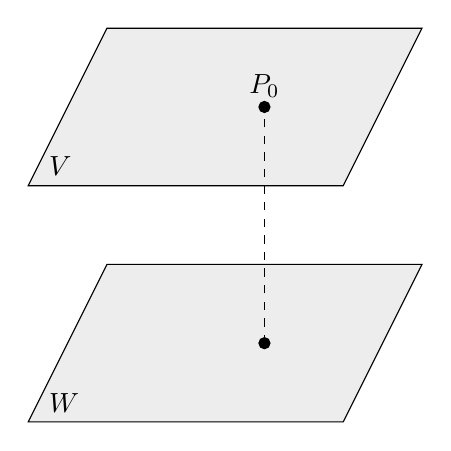
\begin{tikzpicture}
    \filldraw[black!7!white] (0,0) -- (4,0) -- (5,2) -- (1,2) -- cycle;
    \draw (0,0) node[above right,xshift=4pt] {$W$} -- (4,0) -- (5,2) -- (1,2) -- cycle;
    \filldraw[black!7!white] (0,3) -- (4,3) -- (5,5) -- (1,5) -- cycle;
    \draw (0,3) node[above right,xshift=4pt] {$V$} -- (4,3) -- (5,5) -- (1,5) -- cycle;
    %
    \filldraw (3,1) circle (2pt);
    \filldraw (3,4) circle (2pt) node[above] {$P_0$};
    %
    \draw[dashed] (3,1) -- (3,4);
\end{tikzpicture}
}

\begin{examplebox}{}{}
    Los planos $x + 2y - 2z = 3$ y $2x + 4y - 4z = 7$ son paralelos ya que sus vectores normales,
    \begin{matrizn}
        \makecell{\includegraphics[page=8]{Externalizacion/C5/MatricesC5.pdf}}
    \end{matrizn}
    son vectores ortogonales. Encuentra la distancia entre estos planos.

    \tcblower
    \solucion Para encontrar la distancia $D$ entre los planos, podemos seleccionar un punto arbitrario en uno de los planos y calcular su distancia al otro plano. Al establecer $y_0 = z_0 = 0$ en la ecuación $x + 2y - 2z = 3$, obtenemos que $x_0 = 3$ y, por tanto, el punto $P_0$ en este plano. Análogo al ejemplo anterior, la distancia entre $P_0$ y el plano $2x + 4y - 4z = 7$ es
    $$D = \frac{|2(3) + 4(0) + (-4)(0) - 7|}{\sqrt{2^2 + 4^2 + (-4)^2}} = \frac{|6 + 0 + 0 - 7|}{\sqrt{4 + 16 + 16}} = \frac{|-1|}{6} = \frac{1}{6}.$$
\end{examplebox}

\newpage

\section{Proceso de ortonormalización de Gram-Schmidt}

En muchos problemas que involucran espacios vectoriales, quien resuelve el problema tiene la libertad de elegir cualquier base para el espacio vectorial que considere apropiada. En $\RR[n]$, la solución de un problema a menudo puede simplificarse eligiendo una base en la que los vectores sean ortonormales entre sí. En esta sección, mostraremos cómo obtener dichas bases.

En $\RR[2]$, dos vectores ortogonales no nulos son linealmente independientes porque ninguno es múltiplo escalar del otro; y en $\RR[3]$, tres vectores mutuamente ortogonales no nulos son linealmente independientes porque ninguno se encuentra en el plano de los otros dos (y, por lo tanto, no se pueden expresar como una combinación lineal de los otros dos). El siguiente teorema generaliza estas observaciones.

\begin{theorem}{}{ortoindependiente}
    Sean $\mathbb{u}_1$, $\mathbb{u}_2$, $\dots$, $\mathbb{u}_k \in \RR[n]$. Si $\left\{ \mathbb{u}_1, \mathbb{u}_2, \dots, \mathbb{u}_k \right\}$ es un conjunto ortogonal de vectores diferentes del vector cero, entonces dicho conjunto es linealmente independiente.

    \tcblower
    \demostracion Ya que $\left\{ \mathbb{u}_1, \mathbb{u}_2, \dots, \mathbb{u}_k \right\}$ es un conjunto ortogonal, entonces $\mathbb{u}_i \bullet \mathbb{u}_j = 0$, $\forall i \neq j$ con $i, j = 1, 2, \dots, k$. Sea
    $$\mathbb{0} = \alpha_1\mathbb{u}_1 + \alpha_2\mathbb{u}_2 + \cdots + \alpha_k\mathbb{u}_k$$
    con $\alpha_i \in \RR$, debemos probar que $\alpha_i = 0$ para $i = 1, 2, \dots, k$. Así,
    \begin{align*}
        0 = \mathbb{u}_i \bullet \mathbb{0} & = \mathbb{u}_i \bullet \left( \alpha_1\mathbb{u}_1 + \alpha_2\mathbb{u}_2 + \cdots + \alpha_k\mathbb{u}_k \right) \\
        & = \mathbb{u}_i \bullet ( \alpha_1\mathbb{u}_1) + \mathbb{u}_i \bullet (\alpha_2\mathbb{u}_2) + \cdots + \mathbb{u}_i \bullet (\alpha_i\mathbb{u}_i) + \cdots + \mathbb{u}_i \bullet (\alpha_k\mathbb{u}_k) \\
        & = \alpha_1 ( \mathbb{u}_i \bullet \mathbb{u}_1) + \alpha_2 (\mathbb{u}_i \bullet \mathbb{u}_2) + \cdots + \alpha_i (\mathbb{u}_i \bullet \mathbb{u}_i) + \cdots + \alpha_k (\mathbb{u}_i \bullet \mathbb{u}_k) \\
        & = \alpha_1 \cdot 0 + \alpha_2 \cdot 0 + \cdots + \alpha_i \| \mathbb{u}_i \|^2 + \cdots + \alpha_k \cdot 0
    \end{align*}
    Como $\mathbb{u}_i \neq \mathbb{0}$ por hipótesis, $\| \mathbb{u}_i \|^2 > 0$ y se tiene $\alpha_i = 0$ para $i = 1, 2, \dots, k$. Por tanto, $\mathbb{u}_1$, $\mathbb{u}_2$, $\dots$, $\mathbb{u}_k$ son linealmente independientes.
\end{theorem}

